\section{Introduction}

\subsection{The general reconstruction of room layouts} %Problem statement
A reconstruction of a room is the process of taking in some data from a room and transforming it into its 2D floor plan. The floor plan contains basic information, such as the overall shape of the room as well as the location of windows and doors. The spatial dimensions can also be noted down, including the length of a wall or the height of the room. This floor plan is useful in many applications and services, such as virtual room design or simple information gathering in a faster, more convenient way. 

The efficient and precise reconstruction of a room has been attempted numerous
times. The data in most cases is comprised of one or more pictures taken of the room. The process of transformation is the present problem, for which this paper attempts to provide a general solution to. The problems lie in the shape of a given room and how variable any room really is. Given that this problem is solved and the process is complete for any room, many new applications can emerge that utilize this process and make way for new services.


\subsection{The problem with reconstruction of non-cuboid spaces} %Motivation
For most rooms, we can differentiate between cuboid and non-cuboid shaped instances. a cuboid room is regular and rectangular, while a non-cuboid room can have irregular, curved, or non-right-angled surfaces. These differences are presented in Figure [\ref{fig:bothfigures}]. In the realm of cuboid shaped rooms, some progress has been made with the goal of reconstructing. However, there is need for a less restrictive and overall more general process that is able to reconstruct rooms, regardless of shape. Is there maybe a more efficient and general process for reconstruction? This is the question we put the emphasis on in this paper.

\begin{figure}[htbp]
    \centering
    \begin{subfigure}[b]{0.38\textwidth}
        \centering
        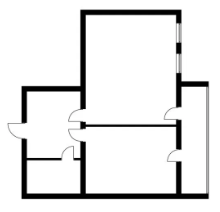
\includegraphics[width=\textwidth]{images/cuboidfloorplan.png}
        \caption{Example of cuboid rooms}
        \label{fig:cuboidroom}
    \end{subfigure}
    \hfill
    \begin{subfigure}[b]{0.38\textwidth}
        \centering
        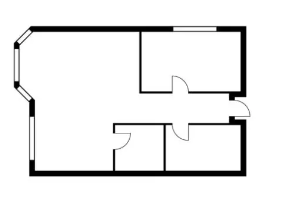
\includegraphics[width=\textwidth]{images/noncuboidfloorplan.png}
        \caption{Example of non-cuboid room (far left)}
        \label{fig:noncuboidroom}
    \end{subfigure}
    \caption{Difference in room shapes}
    \label{fig:bothfigures}
\end{figure}

This is a difficult problem for the following reasons. A room can take on different shapes, the room height can change and in some places the space can even narrow or widen. For this reason it has been proven to be a difficult challenge to efficiently map out a room's floor plan based on images. The difficulty is compounded when relying on one image to extract spatial information. Images provide limited depth perception when taken from a single viewpoint. This also makes the scaling of a processed room difficult to evaluate.
\newpage

\subsection{The Basis of SKBD} %Solution
There are various attempts at resolving the problem of room reconstruction. Most papers in this field are concerned with the reconstruction of cuboid shaped rooms with information given from a single image. As a consequence, these results provide a limited precision on depth and scaling. The most promising papers are given more attention in Related Work[\ref{sec:relatedwork}]

Our presented solution, named Segment Knotting Boundary Detection (abbreviated to SKBD) aims to provide a more versatile method for reconstructing a room. With this paper, the aim was to develop a processing method that can reconstruct a non-cuboid shaped room from a small number of images. The solution can also determine the depth and scale properties of a room, since multiple viewponts are being used. It also puts more emphasis on detecting segments outlined by feature points and local descriptors. 



\subsection{Segment connection} %Contributions
This solution differs from the currently published ones in terms of usage and in terms of the reconstructing process. A heavy focus was put on image segmentation. A segment refer to a part of the image that can be detected and separated. Detecting the connection between segments involves identifying how these segments relate to one another. This could mean determining if they belong to the same structure, if they interact in some way, or if they share common features. SKBD relies on detecting segments in the taken images and then matching them. Using this approach we relied less on the proximity of these segments which in turn resulted in identifying connections that may not be immediately obvious.

%Roadmap
This article will discuss related works [\ref{sec:relatedwork}] in this field, explains the methodology and development process of SKBD, then presents findings about the accuracy of the developed method. It will also draw a conclusion based on the results of the development and talk about potential directions for this method in the future.




